%!TEX TS-program = xelatex
%!TEX encoding = UTF-8 Unicode


\documentclass{Dissertate}

\begin{document}

% the front matter
%!TEX root = ../thesis.tex
% Some details about the dissertation.

\title{Supporting tools for\\\vspace{-1.3cm}Agile software development:\\experience from a real use case}
\author{Ciprian Stefan Voinea}
 
%If you have one advisor
\advisor{Dott. Armir Bujari}

%If you are coadvised
\coadvisorOne{Delightful Researcher}
\coadvisorOneUniversity{Università Blabla}

\mastername{Computer Science}

% \maketitle
% \copyrightpage
\frontmatter
\setstretch{\dnormalspacing}
% \abstractpage
% \tableofcontents
% %\authorlist
% \listoffigures
%\dedicationpage
% \acknowledgments

% \doublespacing

% include each chapter...
\setcounter{chapter}{0}  % start chapter numbering at 1
%!TEX root = ../thesis.tex
\chapter{Introduction}
\label{introduction}

%\hl{introduzione a significato di way of working (in SW)
%	cercare articoli da blog per spiegare
%	martin fowler		
%
%fare tracking delle isssue / bug è diventato difficile / complesso
%	molti tool open source che fanno anche documentazione e code review (altri aspetti)
%
%l'evoluzione negli ultimi anni nelle aziende IT
%	necessità di organizzazione delle azienda e la necessità di avere una gerarchia (o simil gerarchia)
%
%ho sperimentato questo approccio in athonet, mostrata interessata all'utilizzo di un gestionale sw di tipo agile per la gestione dei processi di sviluppo sw interni
%
%I have sperimented ... 
%}

\hl{INTRODUCTION TO WHAT IS A WAY OF WORKING\\HOW IT IS APPLIED IN MODERN SOFTWARE DEVELOPMENT COMPANIES\\THE IMPORTANCE OF HAVING A GOOD WAY OF WORKING FOR A COMPANY IN ORDER TO BE PRODUCTIVE}

\section{Premise}
	This document is a report of the two month curricular internship done between June and July 2019 at Athonet under the supervision of Dr. Fabio Giust.
	It contains a description of the work that I have done and an introduction to Agile and Scrum software developing methodologies.\\
	%todo togliere se non serve
	%todo aggiungere footnote sito dilbert
	To introduce or to describe some of the arguments I will be using some comic strips of Dilbert, a character invented by Scott Adams.
	It satirically represents the problems that can be present in a small or big company of software development.
	\begin{figure}[H]
		\centering
		
\includegraphics[width=1\textwidth]{resources/Dissertate}\\
		\caption[Dilbert, \Quote{Plan A}]{Dilbert, \Quote{Plan A}, Monday June 06, 2011}
	\end{figure}
	The document contains a Glossary section that describes technical words that would need a more specific introduction: these are marked as \gls{Example}.\glsadd{Example}\\
	
\section{The company}
	Athonet is a telecommunication company headquartered nearby Vicenza.
	It stem from the idea that broadband networking should be easily available to people in rural areas and to companies that work in mission critical services or special environments like shipping, mining companies or even hospitals (safety critical).\\
	%todo officially it started senza was?
	%todo aggiungere footnote sito ericsson?
	Officially it was started in 2004, although a working prototype of their idea was already developed by the CEO and CTO that were working alongside in Ericsson at that time.
	%todo inserire citaizione Athonet.com
	\begin{figure}[H]
		\centering
		
\includegraphics[width=.7\textwidth]{resources/ath_logo}\\
		\caption[Athonet's logo]{Athonet's logo}
	\end{figure}
	Low latency communication, reliability and security are at the core of what Athonet provides.
	%todo spiegare significato di LTE prima di introdurlo
	Their main product is PriMo, a device that allows to create a dedicated core network, or enterprise LTE.
	\begin{figure}[H]
		\centering
		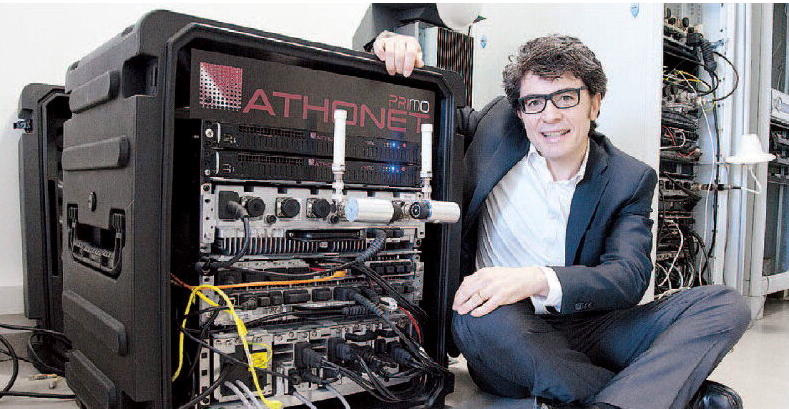
\includegraphics[width=.8\textwidth]{resources/gianluca_primo}\\
		\caption{The CTO, \textit{Gianluca Verin}, with Athonet's main product \textbf{\Quote{PriMo}}\cite{gianluca_primo}}
	\end{figure}
	In 2012, after a disastrous earthquake destroyed all the communication lines in Emilia Romagna, Athonet has reestablished connectivity, thus showing the how PriMo can be used on the field in emergency situations.\\
	Athonet installed PriMo at the top of a school, allowing them to cover the affected area not only for the operators of Servizio Civile but for the citizens as well.\\
	In December 2013, Athonet has been rewarded by Giorgio Napolitano, the then President of the Italian Republic, with a medal for merits for the sustainability in the digital sector.\\
	Lately they have migrated some of their functions to the cloud: by using AWS they have achieved a hybrid product, BubbleCloud, a plug and play solution that allows to locally deploy the physical Edge Nodes while managing them from the AWS cloud.\\
	This small business has much to offer, considering that some of it's competitors are giants like Nokia and Ericsson.\\
	As a proof of the continuous will to improve and for the solution it provides, Athonet has been awarded with four Global Mobile Awards at the GSMA Mobile World Congress, held in February 2019 in Barcelona.
	%todo inserire citazioni
%	https://www.millionaire.it/athonet-la-startup-italiana-che-trionfa-al-mobile-world-congress/#!
%	http://www.ilgiornale.it/news/interni/genio-torna-svezia-soffrire-nella-sua-italia-912407.html

\section{The project}
	It consists in installing and configuring two main software tools, Jira and Confluence, alongside plugins to add more functions and enhance their potentiality.
	However, the most important part of this project is not installing the software, but adapting it to the needs of the company.\\
	As said earlier Athonet my still be small, but it's a growing company, and because of this it needs to give itself some internal rules and specifications to follow when working on a task, communicating with the client or even share internal information to employees.
	Not only for themselves but for clients they work with as well, since most big companies require that their partners have internal regulations, no matter the number of people in the company.\\
	As I will explain in the following chapters Jira is an Issue Tracking System, a software that allows to follow the tasks (like resolving bugs or implementing features) that are related to a project, while Confluence is a software for sharing knowledge, that means sharing internal documents, keeping a wiki, having documentation available and even for customers.\\
	My task was to demonstrate that these tools are what Athonet needs to be a strong an coherent company, where information is always shared and available, while maintaining a history of changes, by creating an environment that suited their needs and that can evolve alongside the company.\\
	To do this I have learned the basics of Agile and Scrum methodologies, how a company operates internally and with their clients and how introducing a new tool may improve the way of working, even if it creates chaos at the beginning.

\section{Document organization}
	This thesis is organized as follows:
	\begin{itemize}
		\item Chapter 1 or \Quote{Introduction}: describes the overall content of this document
		\item Chapter 2 or \Quote{The internship project}: describes in detail the objectives and planning of the internship project
		\item Chapter 3 or \Quote{Agile processes and methodologies}: an introduction to the Agile software development
		\item Chapter 4 or \Quote{Jira and Confluence: the essentials}: describes the most valuable functionalities of Jira and Confluence
		\item Chapter 5 or \Quote{Project implementation}: details how the project has been implemented by dividing it into time periods
		\item Chapter 6 or \Quote{Conclusions}: contains the retrospective of the project, future developments and personal considerations
	\end{itemize}
	

%!TEX root = ../thesis.tex
%\begin{savequote}[75mm]
%Nulla facilisi. In vel sem. Morbi id urna in diam dignissim feugiat. Proin molestie tortor eu velit. Aliquam erat volutpat. Nullam ultrices, diam tempus vulputate egestas, eros pede varius leo.
%\qauthor{Quoteauthor Lastname}
%\end{savequote}

%\chapter{\textsc{The internship project}}
\chapter{The internship project}

%\newthought{There's something to be said} for having a good opening line. Morbi commodo, ipsum sed pharetra gravida, orci  $x = 1/\alpha$ magna rhoncus neque, id pulvinar odio lorem non turpis \cite{Eigen1971, Knuth1968}. Nullam sit amet enim. Suspendisse id velit vitae ligula volutpat condimentum. Aliquam erat volutpat. Sed quis velit. Nulla facilisi. Nulla libero. Vivamus pharetra posuere sapien. Nam consectetuer. Sed aliquam, nunc eget euismod ullamcorper, lectus nunc ullamcorper orci, fermentum bibendum enim nibh eget ipsum. Donec porttitor ligula eu dolor. Maecenas vitae nulla consequat libero cursus venenatis. Nam magna enim, accumsan eu, blandit sed, blandit a, eros.
%$$\zeta = \frac{1039}{\pi}$$

% For an example of a full page figure, see Fig.~\ref{fig:myFullPageFigure}.

This chapter contains the results of the discussions and planning that have been made prior to the beginning of the internship.
These contents are described in more detail in the \Quote{Piano di Lavoro}, a document that contains an estimation of resources for each task that composes the project.\\
At the beginning of May I met with the tutor to understand the needs of the company and draft a plan.
Below I describe how a resolution for the problem was first thought.

\section{The company's needs}
	%todo Forse io scriverei il paragrafo al contrario: ci sono questi needs, e attualmente i software si comportano cosi'. 
	At the time of writing it has nearly 40 employees and it is expected to hire new people soon.\\
	Athonet uses multiple software tools for keeping track of projects, sharing information internally and with the clients, visualizing product roadmaps, etc.\\
	The most important tools they are currently relying on are:
	%todo aggiungere riferimenti a siti ufficiali
	\begin{itemize}
		\item Redmine as an Issue Tracking System
		\item SharePoint as a collaborative platform
		\item Planner for visualizing project roadmaps
		\item GitLab as a repository
	\end{itemize}
	%todo rivedere frase
	While some of these packages are compatible, others were not developed to be used together.
	There are plugins that connect them, but these don't allow much customization and since are made from multiple developers, not always are compatible  a new software release is issued.\\
	There is a need then to provide employees with a suite of stable tools that are easily interconnected and with a vast and well done documentation.
	Also, these tools must be easy to maintain and update, since they don't have to become obsolete and outdated.\\
	Nobody likes legacy systems.
	\begin{figure}[H]
		\centering
		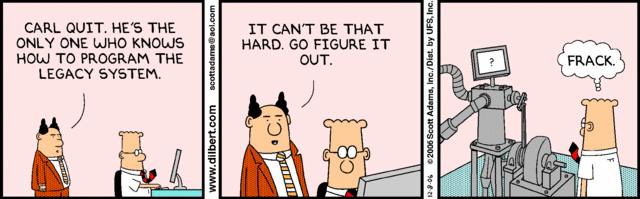
\includegraphics[width=1\textwidth]{resources/legacy-code}\\
		\caption[Dilbert, \Quote{Plan A}]{Dilbert, \Quote{Plan A}, Monday June 06, 2011}
	\end{figure}
	Internal changes may not be directly visible to the clients, but the effect of having a much organized company, where there is always track of the work done and in progress ensures that when there is a request from the client it does not go unseen or unanswered.\\
	Forcing employees to use a software instead of another one though is not easy without creating chaos.
	This is why a good and easy to consult documentation is the key on helping employees transition.

\section{Requirements and objectives}
	%When discussing with the tutor he as explained me the problem step by step and we have set some requirements in order to give them importance and priority.
	The final objective was to create a suitable environment that would work and be ready to transfer it into production and explain the users how to use it.\\
	Requirements can be divided in three categories based on their importance:
	\begin{itemize}
		\item Mandatory (\Quote{Obbligatorio} in italian): that have to be implemented, represent the core of the project;
		\item Desirable (\Quote{Desiderabile} in italian): not mandatory for the final objective but add greater value;
		\item Optional (\Quote{Facoltativo} in italian): add value to the project but not as much as the previous ones, carried out only if there is time left for them.
	\end{itemize}
	Each requirement has a unique ID that is composed by the first letter of their importance (from the italian word to resemble the Piano di Lavoro) and a number.\\
	%todo mettere lista in appendice
	\hl{Here a list of the requirements, as presented in the work plan document:}
	%todo aggiungere tabella con i requisiti

\section{Approaching the problem}

	\hl{How I thought I could approach the problem.
	Write that I have thought of use chases and associate them to the requirement?}

\section{Time division and planning}
	To formalize the time division of the project I have used a Gantt diagram and a table contains a realistic approximation of the hours spent per task.\\
	The internship was planned for ten weeks and the project has been spread such that I could have time to understand the tools and use them so that I could get acquainted.
	This time period also includes the phases for getting feedback from users, fine tune the configuration, explain the tools to various members of the company and, in case of incidents, slack time.\\
	%todo spostare immagine in appendice
	%Difficile da leggere. Magari funziona meglio messo in verticale a pagina intera?
	\begin{figure}[H]
		\centering
		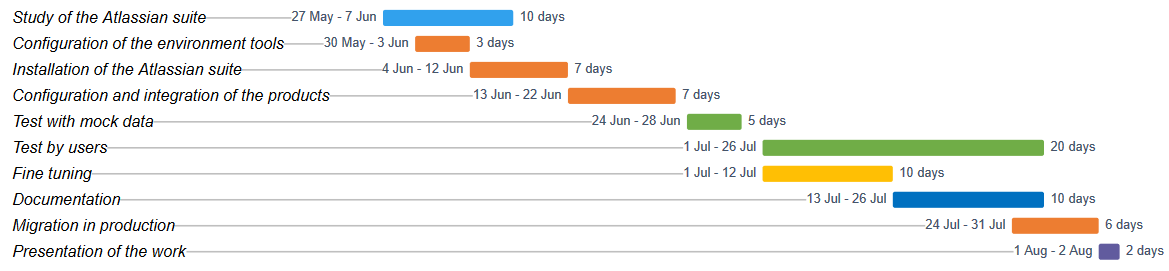
\includegraphics[width=\textwidth]{resources/work_plan_gantt}\\
		\caption{Gantt diagram contained in the ``\textit{Piano di Lavoro}'' document}
	\end{figure}
	I started to create a temporal sequence only after I well understood the requirements and got an idea about how Atlassian's software works, also I wanted to figure out the final objective and thinking how to achieve it.
	% todo spiegare diagramma di gantt?
	\hl{As it can be seen in the Gantt diagram, there are some tasks that overlap in time: for example the Study of the Atlassian suite overlaps with Configuration of the environment tools.
	This because the tasks may have something in common or one helps the achievement of the other.
	While studying the requirements for the Atlassian software I decided I would also configure the host machine.}\\
	I have coarse grained planned four main time periods:
	\begin{itemize}
		\item Learning
		\item Implementing
		\item Testing
		\item Feedback
	\end{itemize}
	Each of these contain smaller tasks that involve studying the tools, installing them and configuring them.\\
	As discussed with the tutor, meetings had to be considered so that I could explain the progress to him and to other company figures that would eventually use the software.\\
	As milestones I considered having a deliverable that could be easily transitioned from the development to the production environment, such as a script that installs and configures the software or a container.
	By definition this must be versionable and with a well written changelog.
	
	
%!TEX root = ../dissertation.tex
\begin{savequote}[75mm]
This is some random quote to start off the chapter.
\qauthor{Firstname lastname}
\end{savequote}

\chapter{Processi e metodologie dell'agile}


Possibile introduzione del tipo "Before getting into what I have concretely achieved / implemented, let's take a better look at what agile is and how it came to be" (overview)

\section{breve storia dell'agile}
cosa c'era prima dell'agile\\
quando dove e perchè c'era la necessità

\section{il manifesto agile}
i 4 punti fondamentali del manifesto agile

\section{i dialetti / cugini dell'agile}
kanban, etc.

\section{applicazioni dell'agile }
modello spotify (+ altre grandi aziende)\\
e le piccole aziende come athonet come fanno? (misto)

\section{utilità agile}
l'agile può andare a completamente sostituire il resto\\
cosa ne pensano gli utenti

\section{che tipo di agile viene utilizzato da athonet}
misto a causa dei pochi dipendenti che hanno ancora una responsabilità ampia all'interno dell'azienda ma pensano che si possa incorporare agile\\
processi di business


%!TEX root = ../thesis.tex
\begin{savequote}[75mm]
\hl{If a team couldn’t be fed with two pizzas, it was too big.}
\qauthor{Jeff Bezos}
\end{savequote}

% https://areomagazine.com/2019/04/10/agile-and-the-software-industrys-ideology-problem/ 
%https://www.softwaretestinghelp.com/agile-manifesto/
%https://www.smartsheet.com/comprehensive-guide-values-principles-agile-manifesto

\chapter{Agile Software Development}
\label{chapter_3}

Before getting into the implementation and adaptation of Jira and Confluence, \hl{let's back up a little} and understand the concept of Agile, a Software Development Life Cycle (or SDLC) model.\\
%todo rivedere per bene
SDLCs did not emerge until the 1960s; they are considered to be the oldest formalization of framework.
%The Space Shuttle program, which operationally launched in 1982, used information and processing technologies from the 1960s.
A SDLC refers to the ensemble of activities that compose a software project.\\
It starts with the concepts of understanding the problem as well as the requirements and it ends with the retirement of the system (when there is no more maintenance) or with the cancellation of the project.\\
Small projects (generally for a single person) have a simpler life \hl{cycle: find the problem and write a program to solve it: once the problem has been solved}, the program can be deleted and forgotten.\\
%todo or in larger problems / solved
In larger projects, that require a team to be developed, there must be some explicit rules to set a higher quality for the software.\\
As activities are assigned to different people, it becomes critical that all participants share a common view of the execution of the project.
A SDLC model is a framework providing the ordering and dependencies of life cycle activities, managing these can be a major impact for a successful project and its duration.\\
For example, a change in requirements during implementation may invalidate a substantial amount of work and delay the delivery of the system by several months.
Different life cycle models prescribe different actions to handle such changes\cite{software_lyfe_cycle}.\\
%https://en.wikipedia.org/wiki/Software_development_process
%todo mettere tra virgolette
There are many SDLCs like Waterfall, Prototyping, Iterative and Incremental Development, Spiral Development, Rapid Application Development, and Extreme Programming. (XP). 
%todo modificare immagine
%Font piccolo nell'immagine e nella didascalia. In principio, il font dovrebbe essere a grandezza costante sia nel testo che nelle immagini
\begin{figure}[H]
	\centering
	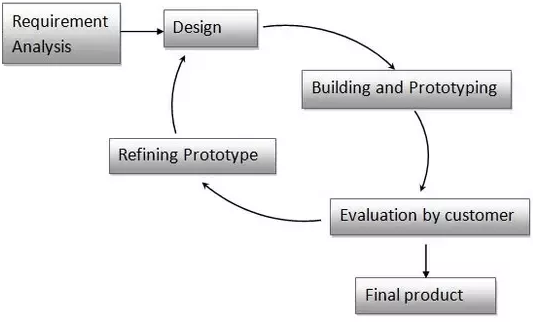
\includegraphics[width=.7\textwidth]{resources/prototype}\\
	\caption{The Prototype model}
\end{figure}
\begin{figure}[H]
	\centering
	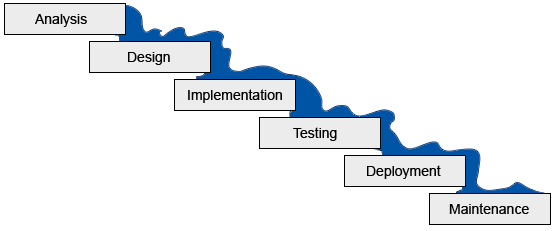
\includegraphics[width=.7\textwidth]{resources/warterfall}\\
	\caption{The Waterfall model}
\end{figure}
%https://www.iso.org/obp/ui/#iso:std:iso-iec:tr:24774:ed-2:v1:en
%todo citare https://www.iso.org/standard/53815.html !!
As the word \Quote{model} suggests, each company may have its own SDLC designed ad hoc for their internal use.\\
This led to the creation of a standard that presents the guidelines for the elements that are most frequently used in describing a process: the title, purpose, outcomes, activities, task and information item.
%todo citare
The ISO/IEC TR 24774:2010: Systems and software engineering -- Life cycle management -- Guidelines for process description\cite{iso_53815}.\\
The complexity and slowness in producing a concrete product in older SDLCs brought the need for a faster and more communicative model.\\
%https://www.tutorialspoint.com/sdlc/sdlc_agile_model.htm
%todo mettere a glossario
%Agile SDLC model is a combination of iterative and incremental process models with focus on process adaptability and customer satisfaction by rapidly and continuously deliver of working software product.
%todo trovare immagine a risoluzione migliore
\begin{figure}[H]
	\centering
	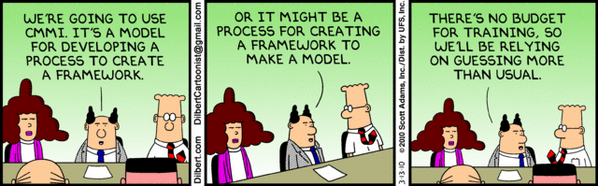
\includegraphics[width=\textwidth]{resources/BffFTn_CAAAEvGn}\\
	\caption{\textit{Redmine}'s logo}
\end{figure}
This chapter describes the most fundamental points of the Agile method, how it started and the adaptations that derived from it, like Scrum.
At the end, it also explains how Athonet's adaptation of the Agile life cycle works.

\section{The need for a new Software Life Cycle}
	The decade of 1990 represented a very important turning point for the digital industry.
	Computers were spreading everywhere and the software companies faced the so-called application development crisis.\\
	The problem was that businesses moved too fast and within the space of three years, requirements, systems, and even entire businesses were likely to change. 
	It meant that a lot of software ended up being incomplete or canceled halfway and the ones that made it through, even if they fulfilled the original objectives of the client, may not meet all the business needs\cite{agility-beyond-history}.
%	https://hackr.io/blog/sdlc-methodologies
	SDLC models can be of two types:
	\begin{itemize}
		\item Iterative: enhances the evolving versions until the complete system is implemented and ready to be deployed
		\item Incremental: the product is designed, implemented and tested incrementally until it is finished
	\end{itemize}
	One of the most characteristic models used before Agile was the Sequential model (or Waterfall).
	The waterfall model became very famous because it has many strong points as:
	\begin{itemize}
		\item Uses clear structure
		\item Determines the end goal early
		\item Transfers information well
	\end{itemize}
	On the other hand, it became obsolete when projects started to be more dynamic and complex.
	Some of it's disadvantages are:
	\begin{itemize}
		\item Makes changes difficult
		\item Excludes the client and/or end user
		\item Delays testing until after completion
	\end{itemize}
	The excessive documentation, the forceful binding to the unchangeable decisions made early in the project and the little communication with the client brought to the need of a new model that prioritizes the product and the stakeholders over bureaucracy.\\
	Those things frustrated people like Jon Kern, an aerospace engineer in the 1990s that with other figures from different industries \Quote{were looking for something that was more timely and responsive}, as he noted.
	He was one of 17 software leaders that started meeting informally and talking about ways to develop software in a simpler way without the excess of documentation and other strict rules.\\
	These talks led to the now famous Snowbird meeting (in Utah, February 2001), when the Agile Manifesto was written down and published.

%
\section{The Agile manifesto}
	The Agile Manifesto is a brief document built on four foundational values and twelve supporting principles for Agile software development\cite{agilemanifesto}.\\
	The four values written on the official website\cite{agile_official} are:
	\begin{itemize}
		\item \textbf{Individuals and interactions} over processes and tools
		\item \textbf{Working software} over comprehensive documentation
		\item \textbf{Customer collaboration} over contract negotiation
		\item \textbf{Responding to change} over following a plan
	\end{itemize}
	The responsiveness of people and embracing the importance of changes are the fundamentals of Agile.
	Although documentation is secondary, it's important to note that Agile streamlines documentation and does not eliminate it.\\
	These twelve principles emphasize things like \Quote{early and continuous delivery of valuable software” and “continuous attention to technical excellence}, and are: 
	\begin{enumerate}
		\item Our highest priority is to satisfy the customer through early and continuous delivery of valuable software.
		\item Welcome changing requirements, even late in development. Agile processes harness change for the customer's competitive advantage.
		\item Deliver working software frequently, from a couple of weeks to a couple of months, with a preference to the shorter timescale.
		\item Business people and developers must work together daily throughout the project.	
		\item Build projects around motivated individuals. Give them the environment and support they need, and trust them to get the job done.
		\item The most efficient and effective method of conveying information to and within a development team is face-to-face conversation.
		\item Working software is the primary measure of progress.
		\item Agile processes promote sustainable development. The sponsors, developers, and users should be able to maintain a constant pace indefinitely.	
		\item Continuous attention to technical excellence and good design enhances agility.
		\item Simplicity--the art of maximizing the amount of work not done--is essential.
		\item The best architectures, requirements, and designs emerge from self-organizing teams.
		\item At regular intervals, the team reflects on how to become more effective, then tunes and adjusts its behavior accordingly.
	\end{enumerate}
	All of them are important but, in my opinion, the ones that add the most value to the Agile line of thought and that differentiate it from the other methods are 2, 4 and 6: they represent the intent of placing the product and the customer above everything else, allowing the use of small informal meetings (even if the decisions should be recorded) and the easy change of requirements because the client is always involved, even as an end user (tester).\\
	Each Agile methodology applies the four values in different ways.
	However, all of them rely on these values to guide the development and delivery of high-quality, working software\cite{4-values-of-the-agile-manifesto}.

\section{Agile's little big cousins}
	While Agile's manifesto contains values and principles, these are not prescriptive.
	In fact the manifesto does not outline specific processes, procedures or best practices.
	The goal is not to develop a rigid framework but rather create a mindset for software development.
	Agile is a blanket term that describes a set of software development principles.\\
	There are many methodologies that derive from Agile's thinking, the most famous ones, according to the annual survey\cite{state-of-agile} from VersionOne's team are:
	\begin{itemize}
		\item Scrum
		\item Scrumban
		\item Kanban
		\item Extreme Programming (XP)
	\end{itemize}
	The essence of Scrum is being agile (fast): a small team that is highly flexible and adaptive.
	\begin{figure}[H]
		\centering
		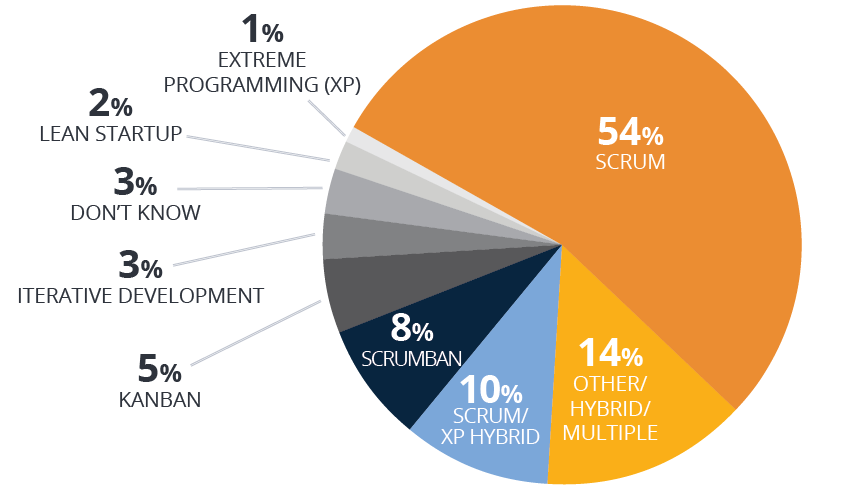
\includegraphics[width=.8\textwidth]{resources/agile-usage-chart}\\
		\caption{The Waterfall and Prototype SDLC models}
	\end{figure}

	%todo modificare immagine
	\begin{figure}[H]
		\centering
		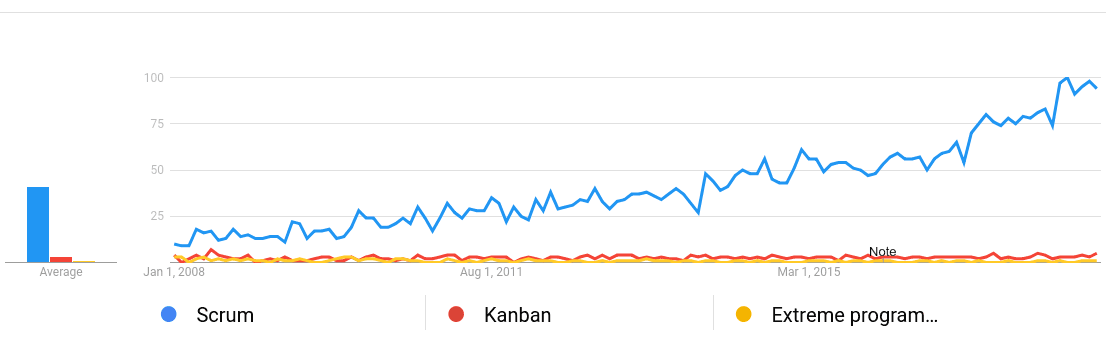
\includegraphics[width=\textwidth]{resources/trends}\\
		\caption{The Waterfall and Prototype SDLC models}
	\end{figure}
	This survey is quite interesting because it provides information from small and big real companies that want to share their experience.
	A very important fact to be noted is that although Technology companies are the ones that mostly participated to the survey, there are other industries that use Agile and are interested in sharing their experience.
	\begin{figure}[H]
		\centering
		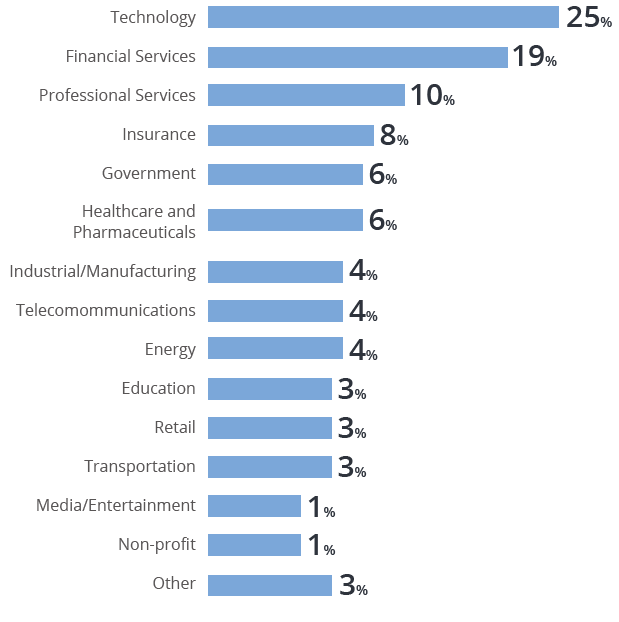
\includegraphics[width=.8\textwidth]{resources/Untitled_2}\\
		\caption{The Waterfall and Prototype SDLC models}
	\end{figure}
	It states that for the year 2018 (which marked their 13th annual report) the reasons for adopting Agile were productivity, improving team morale, reducing product risk (with a lesser percentage than the previous year) and about reducing project costs.\\
	The measures of success mostly cited by the respondents were customer, or user, satisfaction and business value.\\

	%todo Qui devi elencare, e mettere un link alla figura con le percentuali. Il testo dovrebbe contenere tutte le informazioni necessarie per capire il tuo discorso, e le figure servono come chiarimento. Ciascuna figura dovrebbe essere indipendente, nel senso che tra immagine e didascalia si dovrebbe riuscire a capire tutto. 

	According to these companies, the benefits of adopting Agile are:
	\begin{figure}[H]
		\centering
		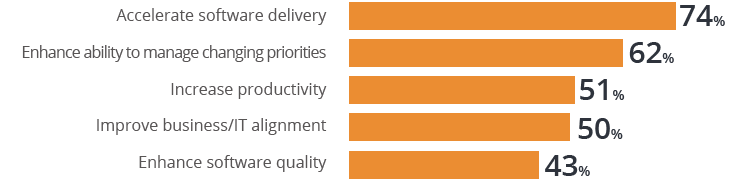
\includegraphics[width=.8\textwidth]{resources/Untitled}\\
		\caption{The Waterfall and Prototype SDLC models}
	\end{figure}

	Also the questionnaire contained a question about what are the recommended Agile project management tools.
	
	%todo modificare immagine
	\begin{figure}[H]
		\centering
		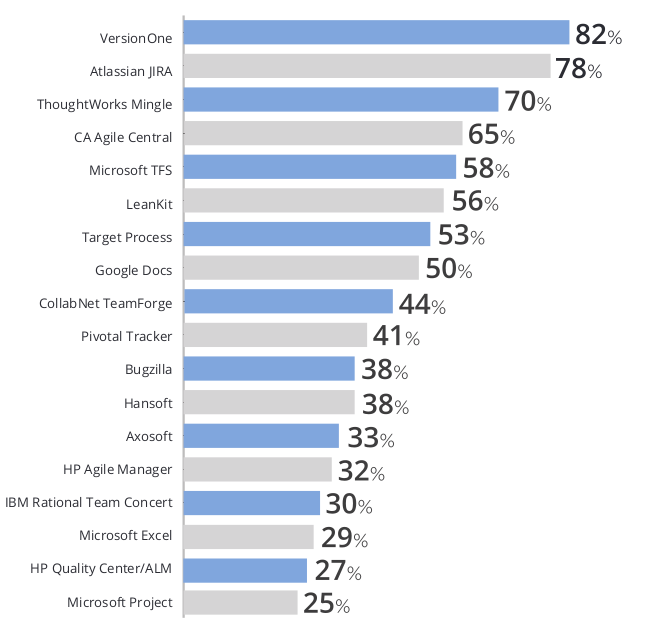
\includegraphics[width=.8\textwidth]{resources/Screenshot}\\
		\caption{The Waterfall and Prototype SDLC models}
	\end{figure}

	As we can see Jira is the second most recommended one.

	\begin{figure}[H]
		\centering
		
\includegraphics[width=.8\textwidth]{resources/Untitled_4}\\
		\caption{The Waterfall and Prototype SDLC models}
	\end{figure}

\section{Agile in practice}
\hl{Briefly describe how some companies use Agile: Spotify / Netflix / Amazon}

% SPOTIFY
%https://medium.com/@media_75624/exploring-key-elements-of-spotifys-agile-scaling-model-471d2a23d7ea
%https://medium.com/productmanagement101/spotify-squad-framework-part-i-8f74bcfcd761

% AMAZON
%https://www.forbes.com/sites/stevedenning/2019/06/02/how-amazon-became-agile/

% MICROSOFT
%https://www.forbes.com/sites/stevedenning/2015/10/27/surprise-microsoft-is-agile/

% NETFLIX
%https://smartbear.com/blog/develop/5-lessons-agile-teams-can-learn-from-netflix/
%http://www.agileadvice.com/2018/03/02/profiles/a-case-study-of-netflixs-high-performance-culture/

%LSD (Lean Software Development)
%This methodology is an adaptation of the Toyota lean manufacturing principles to software development. It was introduced in 2009 by Marry and Tom Poppendieck in their book "Lean Software Development: An Agile Toolkit."

\section{The roles in Agile}
	A distinctive characteristic of the Agile methodology is it's definition of roles: they are not positions, any given person takes on one or more roles and can switch them over time, and any given role may have zero or more people in it at any given point in a project\cite{agileRoles}.
	The ideal team is considered to be composed of five or six people.\\
	These roles are:
	\begin{itemize}
		\item Team leader: team coach or project lead in other methods (Scrum-master e.g.), he is responsible for facilitating the team, obtaining resources for it, and protecting it from problems
		\item Product owner: an executive or key stakeholder, the Product Owner has a vision for the end product and a sense of how it will fit into the company’s long-term goal
		\item Team member: developer or programmer, is responsible for the creation and delivery of a system
		\item Stakeholder: any other person that has direct or indirect interest in the project
	\end{itemize}

%https://www.dummies.com/careers/project-management/agile-project-management-artifacts/
%https://www.atlassian.com/agile/project-management/metrics
%https://www.cognizant.com/services-resources/Services/Cognizant-Agile-Metrics-What-You-Need-to-Want-to-and-Can-Measure.pdf
\section{Time cycles and metrics}
	\hl{COMPLETE}\\
	Scrum teams coordinate development into time-boxed sprints.
	Outside the sprint, teams organize and forecast the amount of work that can be concluded.
	The goal is to have all the forecasted work completed by the end of the sprint.\\
	There are metrics used to track the completion of tasks, these are called burndown reports.
	\begin{figure}[H]
		\centering
		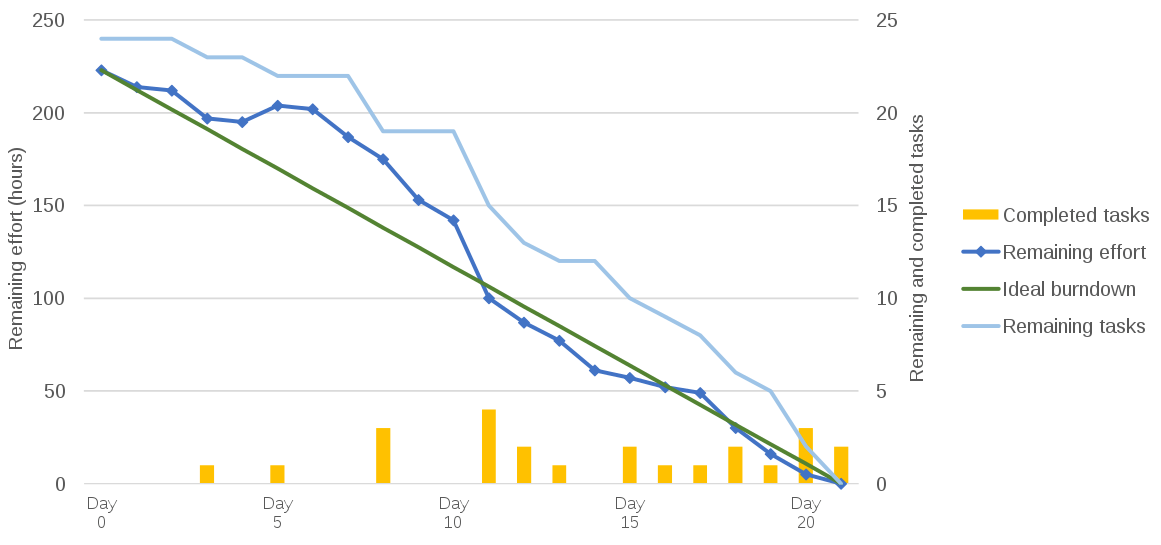
\includegraphics[width=\textwidth]{resources/burndown}\\
		\caption{The Waterfall and Prototype SDLC models}
	\end{figure}
	The x-axis represents time, and the y-axis refers to the amount of work left to complete, measured in either story points or hours.\\
	The sprint is one of the most important time periods in Agile, the other principal ones, according to Atlassian's Agile Coach\cite{epics-stories-themes} are:
	\begin{itemize}
		\item Stories: short requirements or requests written from the perspective of an end user
		\item Epics: large bodies of work that can be broken down into a number of smaller tasks (called stories)
		\item Initiatives: collections of epics that drive toward a common goal
		\item Themes: large focus areas that span the organization
	\end{itemize}
	\begin{figure}[H]
		\centering
		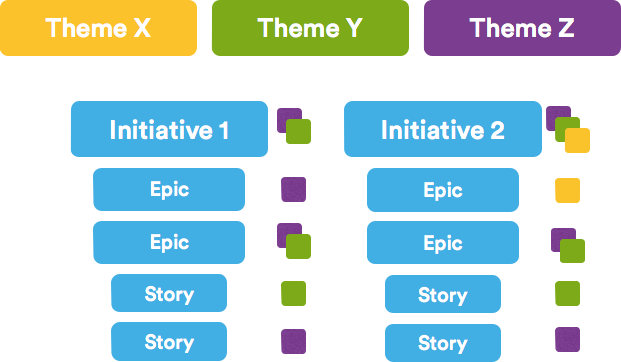
\includegraphics[width=\textwidth]{resources/Themes}\\
		\caption{The Waterfall and Prototype SDLC models}
	\end{figure}
	
%	todo prendere da questo sito https://www.atlassian.com/agile/project-management/epics-stories-themes
	
%https://leankit.com/learn/agile/what-are-the-disadvantages-of-agile/
\section{Disadvantages of Agile Software Development}
	Despite the benefits offered by the Agile model, transition a company's way of working to it is not that easy and if done wrong it may make damage instead of good.
	According to the American entrepreneur Adam Fridman, here are the drawbacks\cite{massive-downside-of-agile} of Agile:
	\begin{enumerate}
		\item Less predictability: developers may not be able to quantify the full extend of the required effort
		\item More time and commitment: a constant interaction, with many face-to-face conversations, is required
		\item Greater demands on developers and clients: extensive user involvement that impacts the quality and success of the project
		\item Lack of necessary documentation: new members that join the team may need more time to understand the project
		\item Project easily falls off track: if a consumer's feedback or communications are not clear, a developer might focus on the wrong areas of development
	\end{enumerate}
	
\section{What Agile variant Athonet uses}
	As many small companies, Athonet will not strictly use one Agile implementation.
	This is also due because of the nature of their product that is not released in simple software patches but it presents itself in a more monolithic version.
	After a research for the available software development life-cycle tools on the market, they chose to try Atlassian's Jira in tandem with Confluence.\\
	As I will say in \Chapref{chapter_5}, the managers liked the idea of Kanban because it allows the employees to come in the morning and choose what they want to work on from the backlog without giving them a two week period of time but letting them complete the tasks in time for the following release.
	But they also liked the idea of having a tool that could transition from a type of project to another in case they want to start applying stricter rules in the future.
	%todo immagine doppia modificare
	\begin{figure}[H]
		\centering
		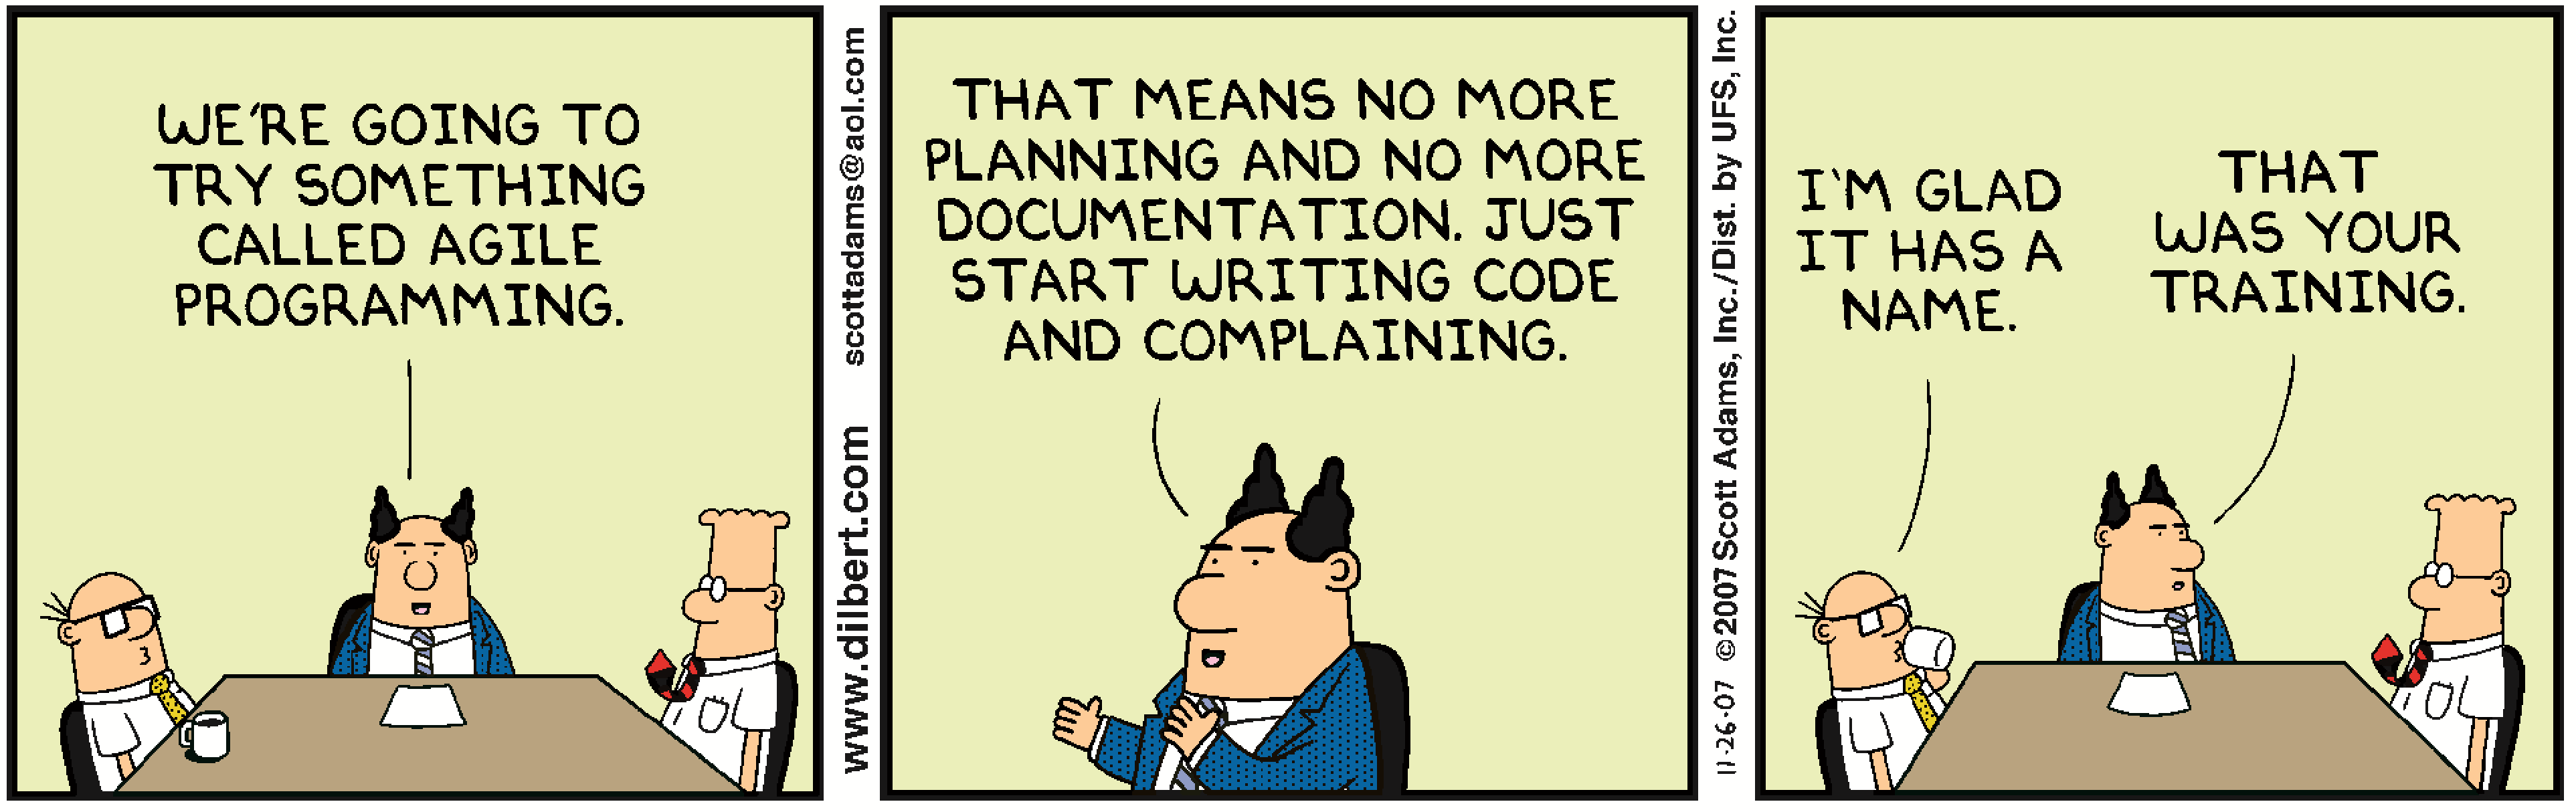
\includegraphics[width=\textwidth]{resources/Dilbert_Training_Agile_Programming}\\
		\caption{The Waterfall and Prototype SDLC models}
	\end{figure}


%!TEX root = ../thesis.tex
\chapter{Conclusions}
\label{conclusions}

After having explained how this solution has been implemented, I would like to draw the conclusions on the project, internship experience and knowledge acquired.

\section{Objectives achievement}
	Even thought the original objectives have changes during the internship, the software's documentation and the blogs presented contained the correct answers in order to correctly configure the software.\\
	Here is a list of the requirements and their status at the end of the project:
	\begin{itemize}
		\item \underline{\textit{O01}}: ACHIEVED
		\item \underline{\textit{O02}}: ACHIEVED
		\item \underline{\textit{O03}}: ACHIEVED
		\item \underline{\textit{O04}}: ACHIEVED
		\item \underline{\textit{O05}}: ACHIEVED
		\item \underline{\textit{D01}}: NOT IMPLEMENTED
		\item \underline{\textit{D02}}: NOT IMPLEMENTED
		\item \underline{\textit{D03}}: ACHIEVED
		\item \underline{\textit{D04}}: NOT IMPLEMENTED
		\item \underline{\textit{D05}}: ACHIEVED
		\item \underline{\textit{D06}}: ACHIEVED
		\item \underline{\textit{F01}}: NOT IMPLEMENTED
		\item \underline{\textit{F02}}: NOT IMPLEMENTED
	\end{itemize} 
	Note that the ones with \Quote{NOT IMPLEMENTED} status is because of internal rules that would not allow interns to interact with the production environment.\\
	Although these have not been achieved, the knowledge on how to implement them has been acquired since their description is contained in the documentation that has been left in Athonet.

\section{Improvement and future implementations}
	As many other projects there are many improvements that can applied.
	To complete the project presented in this thesis I would move it into a production environment and migrate the data from the Redmine instance.
	To have a better and more stable environment thought, there are various improvements that could be made.
	The first and most important one, in my personal opinion, would be separating the database from the Virtual Machine that hosts the software.
	This would bring advantages like: 
	\begin{itemize}
		\item the machine with Jira and Confluence would be less stressed since it would not have so many reads and writes per disk
		\item the database could be stores in a single machine (or multiple ones) with dedicated disks arranged in a redundant way which adds a layer of security, in a disaster recovery plan, over regular backups
		\item maintenance to either one of the machines would be easier and would impact less the company's work
		\item etc.
	\end{itemize}
	Another important improvement would be separating the Confluence instance from the Jira one and, instead of having them running on a dedicated Virtual Machine each, creating a Docker \cite{dock} \gls{container}\glsadd{Container} so that they would be easier to handle (copy, migrate, update).
	\begin{figure}[H]
		\centering
		\includegraphics[width=.4\textwidth]{resources/docker}\\
		\caption{Docker logo}
	\end{figure}
	The use of containers would also allow a better usage of the host machine's resources like memory and CPU power by sharing them.
	These would otherwise be split and left unused by the VMs.
	This kind of improvements should be implemented when planning the migration of the services in a production environment.\\
	Other future improvements can be installing plugins that would allow connectivity with the Microsoft Office suite allowing employees to produce documents and reports without learning how to do it in Confluence and just uploading them.

\section{What I have learned}
	During this internship I had the possibility to better understand the hierarchy of a company, an argument well introduced in the Software Engineering (SWE) course.
	In Athonet I had the possibility to see this first hand and to interact with people on more levels of responsibility, from the CTO, to the product owner to the managers of verification and development teams.\\
	About the tools, it is important to know how to use software like this not only for tracking the status of issues but on how to see other information about them as well.
	This kind of tools are are found in many IT companies, small or big, since they ease not only the work of keeping track of issues but the documentation of meeting notes, internal documents, release changelogs and many other features as well.\\
	In a growing company like Athonet it is useful to set some boundaries, not only for lower level employees like developers, but for the management as well.

\addcontentsline{toc}{chapter}{References}
%\bibliographystyle{unstr}
\bibliography{references}
\cleardoublepage
\phantomsection
\addcontentsline{toc}{chapter}{Acknowledgments}
\acknowledgments


% \clearpage
% \bibliography{references}
% \addcontentsline{toc}{chapter}{References}
% \bibliographystyle{apalike2}

% % !TEX encoding = UTF-8
% !TEX TS-program = pdflatex
% !TEX root = ../tesi.tex

%**************************************************************
% Colophon
%**************************************************************
\clearpage
\phantomsection
\thispagestyle{empty}

\hfill

\vfill

\noindent\myName: \textit{\myTitle,}
\myDegree,
\textcopyright\ \myTime.

\end{document}


%TODO:  page numbering
%todo vedere ordine pagine e pagine da lasciare bianche
%todo mettere copyright?